%%%%%%%%%%%%%%%%%%%%%%%%%%%%%%%%%%%%%%%%%%%%%%%%%%%%%%%%%%%%%%%%%%%%%%%%%%%%
% AGUtmpl.tex: this template file is for articles formatted with LaTeX2e,
% Modified December 2018
%
% This template includes commands and instructions
% given in the order necessary to produce a final output that will
% satisfy AGU requirements.
%
% FOR FIGURES, DO NOT USE \psfrag
%
%%%%%%%%%%%%%%%%%%%%%%%%%%%%%%%%%%%%%%%%%%%%%%%%%%%%%%%%%%%%%%%%%%%%%%%%%%%%
%
% IMPORTANT NOTE:
%
% SUPPORTING INFORMATION DOCUMENTATION IS NOT COPYEDITED BEFORE PUBLICATION.
%
%
%
%%%%%%%%%%%%%%%%%%%%%%%%%%%%%%%%%%%%%%%%%%%%%%%%%%%%%%%%%%%%%%%%%%%%%%%%%%%%
%
% Step 1: Set the \documentclass
%
%
% PLEASE USE THE DRAFT OPTION TO SUBMIT YOUR PAPERS.
% The draft option produces double spaced output.
%
% Choose the journal abbreviation for the journal you are
% submitting to:

% jgrga JOURNAL OF GEOPHYSICAL RESEARCH (use for all of them)
% gbc   GLOBAL BIOCHEMICAL CYCLES
% grl   GEOPHYSICAL RESEARCH LETTERS
% pal   PALEOCEANOGRAPHY
% ras   RADIO SCIENCE
% rog   REVIEWS OF GEOPHYSICS
% tec   TECTONICS
% wrr   WATER RESOURCES RESEARCH
% gc    GEOCHEMISTRY, GEOPHYSICS, GEOSYSTEMS
% sw    SPACE WEATHER
% ms    JAMES
% ef    EARTH'S FUTURE
%
%
%
% (If you are submitting to a journal other than jgrga,
% substitute the initials of the journal for "jgrga" below.)

\documentclass[draft,ms]{agutexSI2019}
%\documentclass[ms]{agutexSI2019}

%%%%%%%%%%%%%%%%%%%%%%%%%%%%%%%%%%%%%%%%%%%%%%%%%%%%%%%%%%%%%%%%%%%%%%%%%
%
%  SUPPORTING INFORMATION TEMPLATE
%
%% ------------------------------------------------------------------------ %%
%
%
%Please use this template when formatting and submitting your Supporting Information.

%This template serves as both a “table of contents” for the supporting information for your article and as a summary of files.
%
%
%OVERVIEW
%
%Please note that all supporting information will be peer reviewed with your manuscript. It will not be copyedited if the paper is accepted.
%In general, the purpose of the supporting information is to enable authors to provide and archive auxiliary information such as data tables, method information, figures, video, or computer software, in digital formats so that other scientists can use it.
%The key criteria are that the data:
% 1. supplement the main scientific conclusions of the paper but are not essential to the conclusions (with the exception of
%    including %data so the experiment can be reproducible);
% 2. are likely to be usable or used by other scientists working in the field;
% 3. are described with sufficient precision that other scientists can understand them, and
% 4. are not exe files.
%
%USING THIS TEMPLATE
%
%***All references should be included in the reference list of the main paper so that they can be indexed, linked, and counted as citations.  The reference section does not count toward length limits.
%
%All Supporting text and figures should be included in this document. Insert supporting information content into each appropriate section of the template. To add additional captions, simply copy and paste each sample as needed.

%Tables may be included, but can also be uploaded separately, especially if they are larger than 1 page, or if necessary for retaining table formatting. Data sets, large tables, movie files, and audio files should be uploaded separately. Include their captions in this document and list the file name with the caption. You will be prompted to upload these files on the Upload Files tab during the submission process, using file type “Supporting Information (SI)”

%IMPORTANT NOTE ON FIGURES AND TABLES
% Placeholders for figures and tables appear after the \end{article} command, after references.
% DO NOT USE \psfrag or \subfigure commands.
%
 \usepackage{graphicx}
 \usepackage{amsmath}
%
%  Uncomment the following command to allow illustrations to print
%   when using Draft:
 \setkeys{Gin}{draft=false}
%
% You may need to use one of these options for graphicx depending on the driver program you are using. 
%
% [xdvi], [dvipdf], [dvipsone], [dviwindo], [emtex], [dviwin],
% [pctexps],  [pctexwin],  [pctexhp],  [pctex32], [truetex], [tcidvi],
% [oztex], [textures]
%
%
%% ------------------------------------------------------------------------ %%
%
%  ENTER PREAMBLE
%
%% ------------------------------------------------------------------------ %%

% Author names in capital letters:
%\authorrunninghead{BALES ET AL.}
\authorrunninghead{BALWADA ET AL.}

% Shorter version of title entered in capital letters:
%\titlerunninghead{SHORT TITLE}
\titlerunninghead{DESIGN \& IMPLEMENTATION MESOSCALE EDDY TRANSPORT}

%Corresponding author mailing address and e-mail address:
%\authoraddr{Corresponding author: A. B. Smith,
%Department of Hydrology and Water Resources, University of
%Arizona, Harshbarger Building 11, Tucson, AZ 85721, USA.
%(a.b.smith@hwr.arizona.edu)}
\authoraddr{Corresponding author: D. Balwada,
Lamont Doherty Earth Observatory, Columbia University.
(dbalwada@ldeo.columbia.edu)}

\renewcommand{\thesection}{S\arabic{section}}
\renewcommand{\thesubsection}{S\arabic{section}.\arabic{subsection}}
\renewcommand{\thefigure}{S\arabic{figure}}
\renewcommand{\thetable}{S\arabic{table}}
\renewcommand{\theequation}{S\arabic{equation}}


\begin{document}


%% ------------------------------------------------------------------------ %%
%
%  TITLE
%
%% ------------------------------------------------------------------------ %%

%\includegraphics{agu_pubart-white_reduced.eps}


\title{Supporting Information for ``Design and implementation of a data-driven parameterization for mesoscale eddy-induced transport. Part 1: Two-layer idealized configurations"}
%
% e.g., \title{Supporting Information for "Terrestrial ring current:
% Origin, formation, and decay $\alpha\beta\Gamma\Delta$"}
%
%DOI: 10.1002/%insert paper number here%

%% ------------------------------------------------------------------------ %%
%
%  AUTHORS AND AFFILIATIONS
%
%% ------------------------------------------------------------------------ %%


% List authors by first name or initial followed by last name and
% separated by commas. Use \affil{} to number affiliations, and
% \thanks{} for author notes.
% Additional author notes should be indicated with \thanks{} (for
% example, for current addresses).

% Example: \authors{A. B. Author\affil{1}\thanks{Current address, Antartica}, B. C. Author\affil{2,3}, and D. E.
% Author\affil{3,4}\thanks{Also funded by Monsanto.}}

\authors{Dhruv Balwada\affil{1}, Pavel Perezhogin\affil{2}, Alistair Adcroft\affil{3} and Laure Zanna\affil{2,4}}



% \affiliation{1}{First Affiliation}
% \affiliation{2}{Second Affiliation}
% \affiliation{3}{Third Affiliation}
% \affiliation{4}{Fourth Affiliation}

\affiliation{1}{Lamont-Doherty Earth Observatory, Columbia University, Palisades, NY, USA}
\affiliation{2}{Courant Institute of Mathematical Science, New York University, New York, NY, USA}
\affiliation{3}{Princeton University, Princeton, NJ, USA}
\affiliation{4}{Center for Data Science, New York University, New York, NY, USA}
%(repeat as many times as is necessary)





%% ------------------------------------------------------------------------ %%
%
%  BEGIN ARTICLE
%
%% ------------------------------------------------------------------------ %%

% The body of the article must start with a \begin{article} command
%
% \end{article} must follow the references section, before the figures
%  and tables.

\begin{article}
\onecolumn



\section{Offline Skill Metrics}
\label{app:offline_skill_metrics}

To evaluate the skill of our ML model in an offline setting we use two main skill metrics. The first is the coefficient of determination or $R^2$ skill, defined as, 
\begin{equation}
    R^2 = 1  - \frac{\overline{(y - \hat{y})^2}}{\overline{(y - \overline{y})^2}},
\end{equation}
$y$ is the truth value and $\hat{y}$ is the prediction. The $\overline{(\cdot)}$ corresponds to average over all samples being considered, which is chosen to be over both flux components from both layers, full spatial domain, and all temporal snapshots in the test data (unless indicated otherwise). The $R^2$ skill will be 1 when prediction is perfect and reduces as prediction gets worse. 

The second metric is the Pearson correlation coefficient, 
\begin{equation}
    C = \frac{\overline{(y - \overline{y})(\hat{y} - \overline{\hat{y}})}}{\sqrt{\overline{(y - \overline{y})^2}\overline{(\hat{y} - \overline{\hat{y}})^2}}},
\end{equation}
which is 1 when the truth and the prediction are perfectly correlated, $-1$ for inverse correlation, and 0 for no correlation.



\section{Eddy driven stream function}
\label{app:eddy_streamfn}

The SGS thickness flux corresponds to a volume flux in a layer ($\mathbf{F}_n$), and the net SGS volume flux below a certain interface can be represented as a stream function \cite{mcdougall2001temporal}: 
\begin{equation}
    \mathbf{\Psi}_{n-1/2} = \sum_{i=N}^n \mathbf{F}_i. %(\overline{\mathbf{u}_i h_i} -  \overline{\mathbf{u}}_i \overline{h_i}),
\end{equation}
Inversely, the SGS thickness flux in any layer can be expressed in terms of these SGS stream function as:
\begin{align}
    \mathbf{F}_n & =  \overline{\mathbf{u}_n h_n} -  \overline{\mathbf{u}}_n \overline{h_n} \\
    %& = \overline{\mathbf{u}_n (\eta_{n-1/2} - \eta_{n+1/2})} -  \overline{\mathbf{u}}_n \overline{(\eta_{n-1/2} - \eta_{n+1/2})} \\
    & = \mathbf{\Psi}_{n-1/2} - \mathbf{\Psi}_{n+1/2} \\
    &  = \delta_n \mathbf{\Psi} 
\end{align}
This streamfunction represents a 2D divergent bolus velocity, $\mathbf{u}_n^* = \delta_n \mathbf{\Psi}/\overline{h_n}$.

While we have presented the problem entirely in terms of thickness fluxes to be used in layered models (section 2), a comparable representation of SGS buoyancy fluxes in terms of a stream function can be done for depth-level models. When representing the SGS buoyancy fluxes in depth-level models, a 3D non-divergent velocity field is constructed using this streamfunction - the quasi-stokes velocity - with no-flow boundary conditions at the top and bottom may be used.  

\section{Interface Diffusion and Gent-McWilliams (GM) Parameterization}
\label{app:GM_param}
This SGS thickness flux in MOM6 is parameterized by the interface diffusion parameterization, which prescribes the eddy driven streamfunction as,
\begin{equation}
    \mathbf{\Psi}^{GM}_{n-1/2} = - \kappa^{GM} \nabla \eta_{n-1/2}, \quad 2 \leq n \leq N.
    \label{eqn:GM_streamfunction}
\end{equation}
% and the corresponding thickness flux would be: 
% \begin{equation}
%     \mathbf{F}^{GM}_{n} = - \kappa^{GM}_{n-1/2} \nabla \eta_{n-1/2} + \kappa^{GM}_{n+1/2} \nabla \eta_{n+1/2},
%     \label{eqn:GM_thickness_flux}
% \end{equation}
In this scheme, the stream function at the top and bottom of the water column are prescribed to be zero ($\mathbf{\Psi}^{GM}_{1/2} = \mathbf{\Psi}^{GM}_{N+1/2} = 0$), which ensures that the sub-grid thickness fluxes do not result in any barotropic SGS volume transport. This parameterization always flattens isopycnal surfaces and reduces APE.  

This parameterization is a close cousin of the Gent-McWilliams parameterization \cite{gent1990isopycnal, gent1995parameterizing}, which is designed for use in z-level models, and also reduces APE of the resolved state. 

%In reality, none of these parameterization assumptions may be completely accurate, and the goal of our work is to improve on this parameterization of sub-grid flux. Here we will use a neural network to parameterize $\mathbf{\Psi}_{n-1/2}$. 

%\textcolor{red}{The assumption of zero $\mathbf{\Psi}$ at the top and bottom is only technically defensible in the interpretation of the coarse resolution model as being representative of the TWA equations mapped to mean depth coordinates. In stacked shallow water model, the natural boundary conditions are of zero streamfunction at vertical side boundaries \cite{killworth2001boundary}.}



%%%%
\section{Velocity Gradient Model (VGM)}
\label{app:VGM}

The velocity gradient model is a structural model, where the goal is to accurately predict the patterns in the SGS forcing.  It is derived based on a Taylor series expansion, and by keeping only the first term of the expansion (see derivation in \citeA{aluie2022effective} or appendix B of \citeA{khani2023gradient}). 


For thickness fluxes, the VGM predicted flux is: 
\begin{equation}
    \mathbf{F}_n^{VGM} = C_{VGM} \triangle_c^2 \nabla \overline{\mathbf{u}}_n \nabla \overline{h}_n
\end{equation}
where 
\begin{equation}
    \nabla \overline{\mathbf{u}}_n = 
    \begin{bmatrix}
        \partial_x \overline{u}_n & \partial_y \overline{u}_n \\
        \partial_x \overline{v}_n & \partial_y \overline{v}_n \\
    \end{bmatrix},
\end{equation} 
\begin{equation}
    \nabla \overline{h}_n = 
    \begin{bmatrix}
        \partial_x \overline{h}_n \\
        \partial_y \overline{h}_n \\
    \end{bmatrix},
\end{equation}
$\triangle_c$ is a coarse-graining scale, and $C_{VGM}$ is a scaling coefficient corresponding to the filter scale. Note that in the presence of topography, we defined our filters such that $\overline{\eta}_b = \eta_b$. So, the sub-grid thickness flux in the bottom layer is just the sub-grid deformable thickness flux. 

Unlike the GM parameterization, the VGM based expression is not guaranteed to the APE reducing, and the impact depends non-linearly on the resolved flow.
%, and so $\mathbf{F}_n^{VGM} = c \triangle^2 \nabla \overline{\mathbf{u}}_n \nabla \overline{h}_n^{deformable}$.

% For calculating the eddy driven stream function, we will need to sum over layers: 
% \begin{equation}
%     \mathbf{\Psi}_{n-1/2} = \sum_{i=N}^n c \triangle^2 \nabla \overline{\mathbf{u}}_i \nabla \overline{h}_i^{deformable},
% \end{equation}
% which is not necessarily zero at the surface. 



%%%%
\section{Rotation to thickness gradient frame}
\label{app:frame_rotate}
In this work we often rotate all directional quantities: SGS flux vectors, the velocity gradient tensor and all thickness gradients, to a thickness gradient frame. 
This thickness gradient frame is defined using a set of orthogonal vectors in the horizontal plane. The first of these vectors,
\begin{equation}
    \hat{\mathbf{T}} = \frac{\nabla \overline{h}_n}{|\nabla \overline{h}_n|} = \frac{\partial_x \overline{h}_n}{|\nabla \overline{h}_n|} \mathbf{\hat{i}} + \frac{\partial_y \overline{h}_n}{|\nabla \overline{h}_n|} \mathbf{\hat{j}},
\end{equation}
points down the thickness gradient. The orthogonal (second) vector, following the right hand rule, is defined as, 
\begin{equation}
    \hat{\mathbf{N}} = \mathbf{\hat{k}} \times \frac{\nabla \overline{h}_n}{|\nabla \overline{h}_n|} = \frac{-\partial_y h_n}{|\nabla \overline{h}_n|} \mathbf{\hat{i}} + \frac{\partial_x h_n}{|\nabla \overline{h}_n|} \mathbf{\hat{j}}.
\end{equation}
The corresponding rotation matrix is defined as
\begin{equation}
    \mathbf{R}_n = 
    \begin{bmatrix}
        \hat{\mathbf{T}} & \hat{\mathbf{N}}
    \end{bmatrix} = 
    \frac{1}{|\nabla \overline{h}_n|}
    \begin{bmatrix}
        \partial_x \overline{h}_n & - \partial_y \overline{h}_n \\
        \partial_y \overline{h}_n & \partial_x \overline{h}_n \\
    \end{bmatrix}.
\end{equation} 
This matrix can be used to rotate vector components and tensor components into the thickness gradient frame. Example, the SGS flux vector components in rotated frame can be diagnosed as 
\begin{equation}
    \widetilde{\mathbf{F}_n} = \mathbf{R}_n^T \mathbf{F}_n,
    \label{eqn:vec_rot}
\end{equation}
and the velocity gradient tensor components in  can be rotated as, 
\begin{equation}
    \widetilde{\nabla \overline{\mathbf{u}}_n} = \mathbf{R}_n^T (\nabla \overline{\mathbf{u}}_n) \mathbf{R}.
\end{equation}

When the operation in Equation \ref{eqn:vec_rot} is applied to the thickness gradient itself, we get the expected result 

\begin{equation}
    \widetilde{\nabla \overline{h}_n} = |\nabla \overline{h}_n| \hat{\mathbf{T}} + 0 \hat{\mathbf{N}},
\end{equation}
 
since this vector does not have any projection orthogonal to the thickness gradient direction by definition.


%(\textcolor{red}{Does this mean that we can make some error in F1, and things will still go fine for PE}.)


\section{ML Model Design Sensitivity}
\label{app:ML_model_sensitivity}
There is a vast range of design choices that need to be made when working with machine learning models and designing parameterizations. For example there can be sensitivity and interdependence on (i) ML model size and architecture (e.g. we chose ANN here), (ii) training data size, (iii) training data source (which idealized simulation is used to train), (iv) learning rate and optimizers, (v) random parameter initialization, (vi) training targets, (vii) norms optimized in loss functions, (viii) input stencil/ domain of influence, (ix) selection of input features etc. It is infeasible to do a complete search over the entire parameter space and some human intuition is often used to guide the design, here we show the impact of some choices that helped guide our decisions. 
%During the initial design development process few choices were randomly sampled, and appropriate changes were made based on human intuition. Some of these choices were then rigorously tested, as shown below.
%%%%
%The design of the model features helps us build our physical knowledge and intuition, and also preconceived biases, into our ML model. 
%In preparation for this study, we tested a wide range of models, as listed here: 
% \begin{itemize}
%     \item $\mathbf{F} = f(\nabla u, \nabla h, \triangle)$ Raw model
%     \item $\mathbf{F}' = f(\nabla u', \nabla h', \triangle)$ Coordinate invariant model
%     \item $\mathbf{F}' = \triangle^2 |\nabla u| f(\nabla u'/|\nabla u|, \nabla h'/|\nabla h|, |\nabla h|)$ Coordinate invariant with non-dimensionalized and range limited inputs
%     \item $\mathbf{F}' = \triangle^2 |\nabla u| f(\nabla u'/|\nabla u|, \nabla h'/|\nabla h|) g(|\nabla h|)$ Coordinate invariant with non-dimensionalized and range limited inputs, and assuming a separable model
%     \begin{itemize}
%         \item $g(|\nabla h|) = |\nabla h|^\alpha$, $\alpha=1$ Polynomial form.
%         \item $g(|\nabla h|)$ is learnt.
%     \end{itemize}
% \end{itemize}

%\textbf{Raw Model} This model is relatively simple. However, it struggles to work across filter scales and layers, since the output data varies quite significantly in magnitude and the loss function will end up not being able to learn properties for the data that is in the smaller range of values. \textbf{Coordinate invariant model} The behavior of this model is similar to the raw model, since the range variability of outputs is still quite large. 

\subsection{Impact of different network sizes}
\label{app:ML_model_sensitivity/size}
We want the most skillful predictions at the lowest cost (least number of operations per evaluation of the ANN). We expect that the skill will increase with increasing the number of trainable parameters, but likely saturate beyond a certain point as there may be no more predictive power in the input features left to be extracted. 
In Figure \ref{fig:compare_model_size} we quantify this behavior for one particular class of models (these were trained with following choices: trained using data from the double gyre experiment, where all the data was rotated to the thickness gradient frame. Non-dimensional velocity and thickness gradients were used as inputs. Mean absolute error was used for the loss, with dimensional fluxes (equation 4) as output targets. Both inputs and outputs were normalized using order of magnitude estimates. We used the model snapshots 0-640 for training, 672-736 for evaluation and 736-800 for testing. Adam optimizer was used with a learning rate of 0.01, and training was continued till the relative improvement in the loss saturated within a relative tolerance of 0.01 (1\% error) for at least 10 epochs). 

The model skill, measured as the $R^2$ value, improves as the number of parameters increase, and this is particularly apparent at larger filter scales and when the model stencil is wider. However, since skill is already very high at filter scales of 50 and 100~km this effect is minor, and at larger filter scales the skill seems to asymptote to its maximum value approximately around $10$K parameters.


\begin{figure}
\noindent\includegraphics[width=\textwidth]{figures/comparing_model_sizes_across_scale.pdf}
\caption{ML model skill, defined as the $R^2$ value, as a function of number of parameters for different filter scales. The details ML model being tested is described in \ref{app:ML_model_sensitivity/size}.}
\label{fig:compare_model_size}
\end{figure}


\subsection{Impact of training data size}
To test the impact that the amount of training data has, we experimented with the same setup as the one used in the previous section with varying amount of data. We fixed all aspects, and performed the test in the case where the stencil size is $3\times3$ and ML model has 3386 parameters (model shape 54,36,36,2). 
We created batches of 16 model snapshots, and tested the effect that increasing the number of batches had. As shown in Figure \ref{fig:impact_training_data} the model skill increases up to about 128 batches (2048 model snapshots), but saturates past that point. This led us to use this data volume for training the model used in the main text.

 \begin{figure}
\noindent\includegraphics[width=\textwidth]{figures/impact_training_data.pdf}
\caption{ML model skill, $R^2$ and correlation, as a function of filter scales for different number of data batches used for training.}
\label{fig:impact_training_data}
 \end{figure}

\subsection{Impact of different loss functions and targets}
\label{app:ML_model_sensitivity/loss_func}
Non-dimensionalization of the sub-grid fluxes leads to a significant collapse in the distributions (see Figure \ref{fig:dist_outputs}), but also produces outliers (due to possibility of division by small velocity or thickness gradients). We have two choices of loss during training, either training on the dimensional fluxes $\mathcal{L}^{dim} = || \mathbf{F} - \mathbf{F}^{pred}|| = || \mathbf{F} - (\triangle^2|\nabla\mathbf{u}||\nabla h|) \mathbf{f}_{\theta}()||$ or training on non-dimensional fluxes $\mathcal{L}^{non-dim} =  || \mathbf{F}/(\triangle^2|\nabla\mathbf{u}||\nabla h|) - \mathbf{f}_{\theta}()||$, where $|| \cdot ||$ implies norm that may correspond to mean square error (MSE) or mean absolute error (MAE) in our work. Both these forms should give us the same numerical mapping if a unique function $\mathbf{f}_{\theta}()$ exists, but in the more realistic situation where $\mathbf{f}_{\theta}()$ is an approximation and we want it to equally balance data coming from many regimes (different simulations, varying energy levels at different depths, etc) it would seem that $\mathcal{L}^{non-dim}$ might be a better choice. 
Along with this we also compared the use of MSE vs MAE, since MAE is generally considered to be more tolerant to outliers. 

As seen in Figure \ref{fig:impact_loss_style}, the impact of these choices is relatively minor in the model considered in the previous section. Generally, the models trained using MAE perform better, except at the largest filter scales, where the model trained using non-dimensionalized outputs and MSE does better. However, this latter model is the worst performer at all other scales. The models trained using MAE also generally perform well across a wide range of scales (see bottom panel). To our surprise, the impact of this choice was smaller than expected. For the main study, we used $\mathcal{L}^{non-dim}$ along with MAE.


 \begin{figure}
\noindent\includegraphics[width=\textwidth]{figures/impact_loss_style.pdf}
\caption{Top row shows the model skill in terms of $R^2$ and correlation as a function of filter scale for different choices of loss function. Bottom two rows show the relative error, which is defined as the power spectrum of the (truth - prediction) divided by the power spectrum of the truth; value of greater than 1 implies that the variance in the anomaly field is greater than in the truth. 
}
\label{fig:impact_loss_style}
 \end{figure}

\subsection{Impact of choice of training data}
We want to build ML models that are easily generalizable and training data agnostic. For example, a model trained on data from the Phillips-2-Layer simulation should be able to make good predictions on data from Double-Gyre experiment, and vice versa. Developing appropriate non-dimensionalizations, as highlighted in section 3, is a step in this direction. In Figure \ref{fig:impact_training_exp} we show that the model trained using data from both simulations simultaneously generally performs the best or close to the best, which is why we chose this training strategy for the model in the main text. 

It is worth noting that in fact even models trained on a single experiment perform relatively well when tested on the other experiment. This is a result of the design choices we made. During the initial phase of our development, when we trained models to have the form of equation \ref{eqn:gen_ML_func}, the skill on unseen data was extremely poor (not shown); also see \citeA{perezhogin2025generalizable}.

 \begin{figure}
\noindent\includegraphics[width=0.9\textwidth]{figures/impact_training_exp.pdf}
\caption{Top two rows show the model skill in terms of $R^2$ and correlation as a function of filter scale for different choices of training datasets. 
Bottom two rows show the relative error, which is defined as the power spectrum of the (truth - prediction) divided by the power spectrum of the truth; value of greater than 1 implies that the variance in the anomaly field is greater than in the truth. 
The title of the panels indicate the dataset on which testing is done, and the legend indicated the dataset that is used for training.}
\label{fig:impact_training_exp}
 \end{figure}

\subsection{Impact of other aspects}

The random seed, which sets \textbf{the random initializations} of the ML model weights, seems to have a small impact on the skill. The model skill averaged across all filter scales, for the case discussed in the above section, varied between values of 0.7 - 0.725 over different random seeds. Since this effect seems small, in the main text we use only a single trained model. 


The \textbf{learning rate}, similarly has a minor impact on the final skill but impacts the nature of decrease in the loss. Large learning rates ($\sim 0.1$) lead to noisy training, while smaller rates ($<0.005$) take too many epochs to train. We found than a learning rate around 0.01 was optimal in not taking too many epochs and not being too noisy, which is what we used for the models discussed in the main text. 

\section{Simulation evaluation metrics}
\label{app:online_metrics}
Here we describe the metrics used to assess the physical properties of our simulations. 

\subsection{Overturning Circulation}
The overturning circulation ($\overline{V}_n (y)$) is defined as the volume transport across a longitude band in a particular layer,
 
\begin{equation}
    \overline{V}_n (y) = \oint \overline{v_nh_n}^t dx + \oint \overline{F^y_n}^t dx,
\end{equation}
 
where $F^y_n(x,y,z,t)$ is the sub-grid or sub-filter meridional flux in layer $n$, $\oint (.) dx$ corresponds to a zonal integral over the full longitudinal domain, and $\overline{(.)}^t$ indicates a time average. The first term on the right hand side corresponds to the resolved overturning and includes the contribution from both the mean and the variable parts of the flow, and the second term corresponds to the parameterized overturning. 

\subsection{Eddy Kinetic Energy Spectrum}
The EKE spectrum provides an effective measure of the flow variability at different scales. 
Here, we define it as the zonal wavenumber ($k$) power spectrum of the $\mathbf{u}'_n(x,y,t) = \mathbf{u}_n(x,y,t) - \overline{\mathbf{u}}^t_n(x,y)$, 
 
\begin{equation}
    EKE_n(k) = \frac{1}{2}(\overline{|u'_n(k, y,t)|^2}^{t,y} + \overline{v'_n(k, y,t)|^2}^{t,y}),
\end{equation}
 
where $\overline{(.)}^{t,y}$ is a time and meridional average and $u'_n(k, y,t)$ is the zonal Fourier transform of $u'_n(x, y,t)$. By Parseval's theorem we have
 
\begin{equation}
    \sum_k EKE_n(k) = \frac{1}{2} \int ( \overline{u'_n(x, y,t)^2}^{t,y} + \overline{v'_n(x, y,t)^2}^{t,y}) dx,
\end{equation} 
 
which shows the scale-wise decomposition aspect of the zonal wavenumber EKE spectrum in the $x$-direction. We used the xrft package \cite{xrft} for this analysis. 
When using xrft with non-periodic data, we use a Hann window and select a region with relatively homogeneous statistics --- for Double-Gyre simulation we compute spectral metrics over 5-17$^o$ Longitude and 32-43$^o$ Latitude.


\subsection{Integral Kinetic and Available Potential Energies}
The volume integrated KE in Joules is defined as:
 
\begin{equation}
    KE = \frac{1}{2} \sum_k \int \rho_0 |\mathbf{u}_k|^2 h_k dx dy.
\end{equation}
 
The $KE$ of the mean flow ($\overline{\mathbf{u}_k}^t$, $\overline{h_k}^t$) is referred to as $MKE$, and the $EKE$ is defined as $EKE = \overline{KE}^t - MKE$. 

The volume integrated APE in Joules is defined as: 
 
\begin{equation}
    APE = \frac{1}{2} \sum_k \int \rho_0   g'_{k-1/2} (\eta_{k-1/2} - \eta^{ref}_{k-1/2})^2 dxdy.
\end{equation}
 

The $MAPE$ is the $APE$ of the mean state ($\overline{\eta_{k-1/2}}^t$), and the $EAPE$ is given by $EAPE = \overline{APE}^t - EAPE$.

For filtered and coarsened flow ($\overline{\mathbf{u}_k}^{\triangle}$, $\overline{h_k}^{\triangle}$) we can also define the total kinetic energy ($KE^\triangle$), which has its corresponding mean ($MKE^\triangle$, for $\overline{\mathbf{u}_k}^{\triangle, t}$, $\overline{h_k}^{\triangle,t}$) and eddy ($EKE^\triangle$) components. Accordingly, we also define the SGS kinetic energies for the total ($KE- KE^\triangle$), mean ($MKE- MKE^\triangle$), and eddy ($EKE- EKE^\triangle$) flow. Similarly APE and its components can be defined for the filtered and coarsened flow and the SGS contribution.


\subsection{Available potential energy tendency due to sub-filter or parameterized fluxes}
\label{app:online_metrics/APE_tend}
Following \citeA{loose2023comparing}, we can compute the impact that the SGS fluxes have on volume integrated APE tendency as, 
 
\begin{equation}
    (\partial_t APE)^{SF} = \sum_{n=1}^{N} \rho_0 \mathbf{F}_n \cdot \nabla M_n,
\end{equation}
 
where $\mathbf{F}_n$ are the SGS fluxes and $M_n$ is the resolved dynamic pressure. 

In a 2 layer fluid we  have, 
 
\begin{equation}
    (\partial_t APE)^{SF} = \rho_0 g^r_{1/2} (\mathbf{F}_1 + \mathbf{F}_2) \cdot \nabla \eta_{1/2} +  \rho_0 g^r_{3/2} \mathbf{F}_2 \cdot \nabla \eta_{3/2}.
\end{equation}
 
Notably, only the last term on the right hand side, which arises due to SGS fluxes in the bottom layer, makes a significant contribution to the APE tendency, since $|\nabla \eta_{3/2}| \gg |\nabla \eta_{1/2}|$. The barotropic contribution to APE, first term on right hand side, is small. 

We decompose this tendency into the time mean and eddy contribution, by defining the contribution from the mean as  
 
\begin{equation}
    (\partial_t APE)^{SF, mean} = \rho_0 g^r_{3/2} 
 (\overline{\mathbf{F}_2}^t \cdot \nabla \overline{ \eta_{3/2}}^t),
\end{equation}
 
where the barotropic contribution is neglected. The eddy contribution is defined as $(\partial_t APE)^{SF, eddy} =\overline{(\partial_t APE)^{SF}}^t-(\partial_t APE)^{SF, mean}$.


\section{Online sensitivity to grid-size and parameterization coefficients}
\label{app:online_sensitivity}

Simulation of oceanic mesoscale turbulence is relatively sensitive to how well the first baroclinic deformation radius (shown in Figure \ref{fig:Rd} for the two simulations considered here) is resolved. In this study we chose our coarsening scale and simulation grid-size to lie in a range that encompasses the deformation radius, so that skill of the new parameterization at both the eddy permitting and non-eddying resolutions can be investigated. Here we provide details of the sensitivity of the coarse simulations to both grid spacing and parameterization coefficients. 

\subsection{Phillips-2-Layer}
For Phillips-2-Layer simulation we tested the sensitivity of the overturning transport to the grid size and parameterization coefficients,  shown in Figure %\ref{fig:P2L_sensitivity} and 
\ref{fig:P2L_sensitivity_detail}. 

In this case, the unparameterized low resolution simulation always has lower overturning transport relative to the HR simulation. The response of the parameterized flux contribution to the GM diffusivity is almost linear and insensitive to grid size, and adjusting the GM diffusivity allows us to increase the total overturning transport to the appropriate value. However, this is only achieved when the diffusivity is relatively large ($\kappa_{GM}\sim 8,000-10,000$~m$^2/$s), which is also a parameter regime in which the resolved eddying flow has been entirely suppressed. Consequently the contribution of the resolved flow to the overturning has been completely eliminated and the entire contribution comes from parameterized fluxes (Figure \ref{fig:P2L_sensitivity_detail} second column). There seems to be no lower diffusivity value at which the appropriate overturning can be achieved with only marginal impact to the resolved flow. 

In contrast, the simulations with the ANN based parameterization are usually able to achieve the appropriate level of overturning with minimal damage to the resolved flow. The response of the parameterized flux to the grid size and parameterization amplification coefficient ($C_{ANN}$) is non-linear. At grid sizes of 10 and 20~km, which are smaller than the deformation radius everywhere in the domain, the appropriate overturning is achieved at $C_{ANN}=1$ and with minimal damage to the resolved overturning. At a grid size of 80~km, which is larger than the deformation radius everywhere in the domain, the appropriate overturning is achieved at $C_{ANN}=2$. At the intermediate grid size of 40~km, the ANN parameterization does produce improvements to overall overturning with little damage to the resolved flow (also at $C_{ANN}=1$), but is unable to achieve similar overturning to the HR simulation. We anticipate that combining the thickness flux parameterization with a momentum flux parameterization may be able to produce further improvements at these intermediate resolutions. 



\subsection{Double-Gyre}
Unlike the Phillips-2-Layer simulation, in the Double-Gyre case there is no overturning circulation. In the context of the thickness flux parameterization, the error in the MAPE is the most relevant, which is also linked to the error in mean SSH. We tested the sensitivity of these quantities and a few others to the parameterization coefficients and grid-size (Figure \ref{fig:DG_sensitivity}). 

For the GM parameterization, a diffusivity of about $200\;m^2/s$ is able to achieve the appropriate MAPE at all resolutions, which similar to the Phillips-2-Layer also comes an almost complete damping of the resolved eddies. The ANN is able to achieve the best MAPE with $C_{ANN}\sim 0.5-0.75$, and this happens with relatively less deterioration in the resolved eddies.

\begin{table}[ht]
    \centering
    \renewcommand{\arraystretch}{1.2}
    \begin{tabular}{|c|cc|cc|}
        \hline
        $\triangle_c$ [km]
        & \multicolumn{2}{c|}{$\kappa_{GM}$ [m$^2$/s]} 
        & \multicolumn{2}{|c|}{$C_{VGM}$ [nondim]} \\
        \hline
        & \textbf{P2L} & \textbf{DG} & \textbf{P2L} & \textbf{DG} \\
        \hline
        10  & 137   & 40   & 0.110 & 0.075 \\
        20  & 596   & 105  & 0.077 & 0.072 \\
        40  & 2287  & 192  & 0.077 & 0.067 \\
        80  & 6266  & 108  & 0.091 & 0.048 \\
        \hline
    \end{tabular}
    \caption{Estimated GM diffusivity ($\kappa_{GM}$) and VGM coefficient ($C_{VGM}$) from the data using least squares fitting, for both the Phillips-2-Layer (P2L) and Double-Gyre (DG) setups.}
    \label{tab:gm_vgm_estimates}
\end{table}




 \begin{figure}
    \centering
    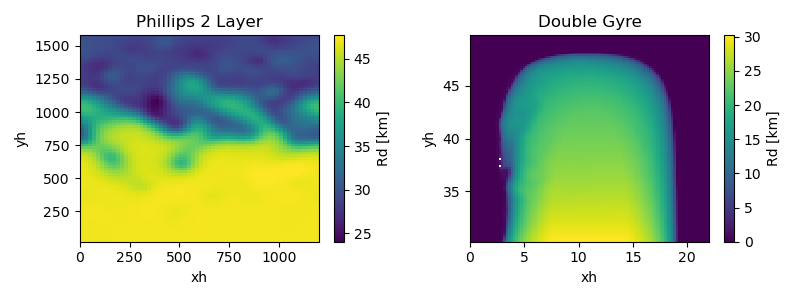
\includegraphics[width=\linewidth]{figures/SI_figures/Def_radii.png}
    \caption{First baroclinic deformation radii for Phillips-2-Layer (left) and Double-Gyre (right). Note the different range of scales for the two colobars.}
    \label{fig:Rd}
 \end{figure}

%  \begin{figure}
%     \centering
%     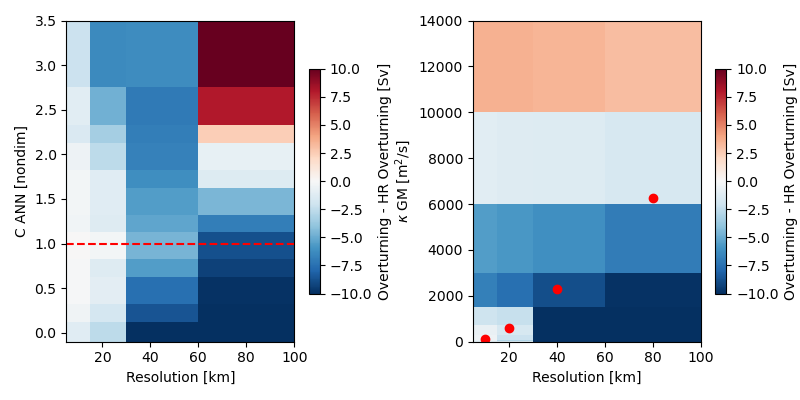
\includegraphics[width=1.0\linewidth]{figures/sensitivity_P2L.png}
%     \caption{Sensitivity of the overturning circulation to the ANN coefficient (left) and the GM diffusivity (right) for the Phillip 2 layer simulations at different resolutions. The dashed red line and red dots correspond to the optimal choice of these parameters suggested based on the offline analysis. }
%     \label{fig:P2L_sensitivity}
%  \end{figure}

 \begin{figure}
    \centering
    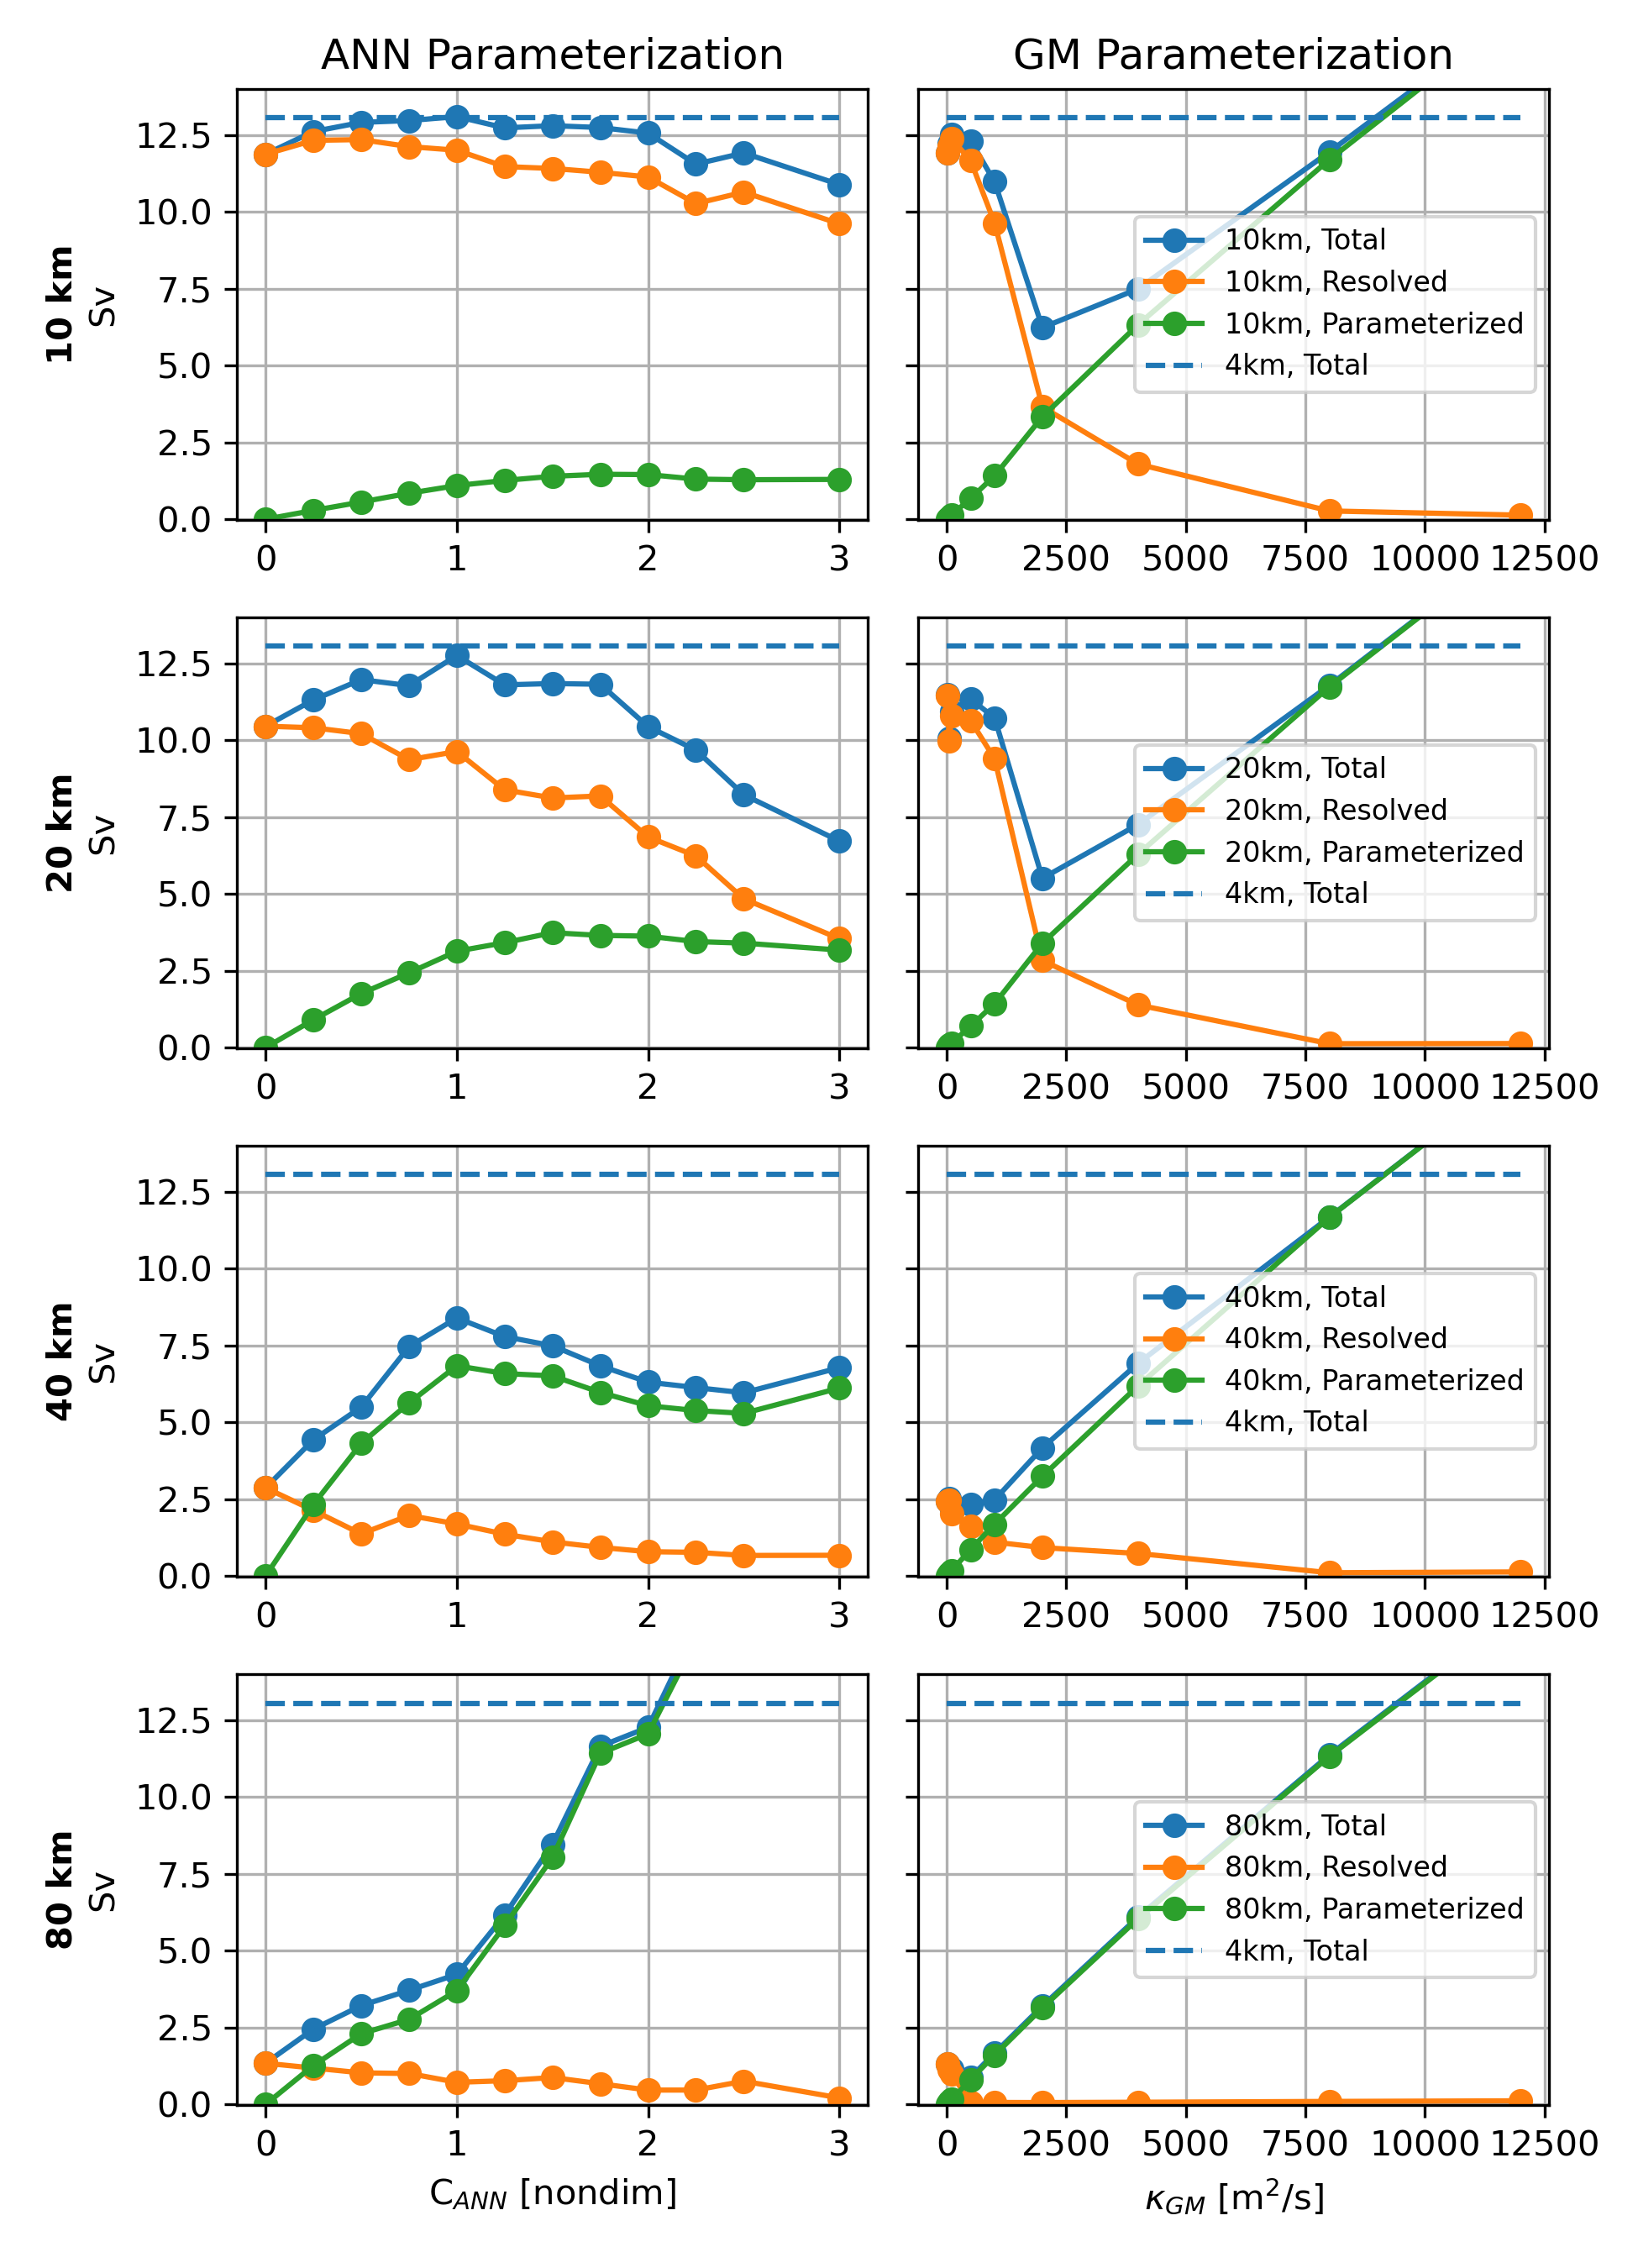
\includegraphics[width=0.9\linewidth]{figures/sensitivity_P2L_multirow.png}
    \caption{Sensitivity of the overturning circulation and its resolved and parameterized components to the ANN coefficient (left) and the GM diffusivity (right) for the Phillip 2 layer simulations at different grid-sizes.}
    \label{fig:P2L_sensitivity_detail}
 \end{figure}

 \begin{figure}
    \centering
    \includegraphics[width=0.9\linewidth]{figures/SI_figures/DG_model_comparison.pdf}
    \caption{Sensitivity to the ANN coefficient (left) and the GM diffusivity (right) for the Double-Gyre simulations at different resolutions.}
    \label{fig:DG_sensitivity}
 \end{figure}




%% ------------------------------------------------------------------------ %%
%
%  END ARTICLE
%
%% ------------------------------------------------------------------------ %%
\end{article}
\clearpage


\bibliography{references}




\end{document}

\noindent\textbf{Contents of this file}
%%%Remove or add items as needed%%%
\begin{enumerate}
\item Text S1 to Sx
\item Figures S1 to Sx
\item Tables S1 to Sx
%if Tables are larger than 1 page, upload as separate excel file
\end{enumerate}
\noindent\textbf{Additional Supporting Information (Files uploaded separately)}
\begin{enumerate}
\item Captions for Datasets S1 to Sx
\item Captions for large Tables S1 to Sx (if larger than 1 page, upload as separate excel file)
\item Captions for Movies S1 to Sx
\item Captions for Audio S1 to Sx
\end{enumerate}

\noindent\textbf{Introduction}
%Type or paste your text here. The introduction gives a brief overview of the supporting information. You should include information %about as many of the following as possible (when appropriate):
% 1. a general overview of the kind of data files;
% 2. information about when and how the data were collected or created;
% 3. a general description of processing steps used;
% 4. any known imperfections or anomalies in the data.

%\clearpage

%Delete all unused file types below. Copy/paste for multiples of each file type as needed.
\noindent\textbf{Text S1.}
%Type or paste text here. This should be additional explanatory text, such as: extended descriptions of results, full details of models, extended lists of acknowledgements etc.  It should not be additional discussion, analysis, interpretation or critique. It should not be an additional scientific experiment or paper.
%
%Repeat for any additional Supporting Text

%%Enter Data Set, Movie, and Audio captions here
%%EXAMPLE CAPTIONS

\noindent\textbf{Data Set S1.} %Type or paste caption here.
%upload your dataset(s) to AGU's journal submission site and select "Supporting Information (SI)" as the file type. Following naming %convention: ds01.

%Repeat for any additional Supporting data sets

\noindent\textbf{Movie S1.} %Type or paste caption here.
%upload your movie(s) to AGU's journal submission site and select, "Supporting Information %(SI)" as the file type. Following naming convention: ms01.

%Repeat any additional Supporting movies

\noindent\textbf{Audio S1.} %Type or paste caption here.
%upload your audio file(s) to AGU's journal submission site and select "Supporting Information %(SI)" as the file type. Following naming convention: auds01.


%Repeat for any additional Supporting audio files

%%% End of body of article:
%%%%%%%%%%%%%%%%%%%%%%%%%%%%%%%%%%%%%%%%%%%%%%%%%%%%%%%%%%%%%%%%
%
% Optional Notation section goes here
%
% Notation -- End each entry with a period.
% \begin{notation}
% Term & definition.\\
% Second term & second definition.\\
% \end{notation}
%%%%%%%%%%%%%%%%%%%%%%%%%%%%%%%%%%%%%%%%%%%%%%%%%%%%%%%%%%%%%%%%


%% ------------------------------------------------------------------------ %%
%%  REFERENCE LIST AND TEXT CITATIONS

%%%%%%%%%%%%%%%%%%%%%%%%%%%%%%%%%%%%%%%%%%%%%%%
% 
%
% \bibliography{<name of your .bib file>} do not specify file extension
%
% no need to specify bibliographystyle
%
% Note that ALL references in this supporting information file must also be referenced in the primary manuscript
%
%%%%%%%%%%%%%%%%%%%%%%%%%%%%%%%%%%%%%%%%%%%%%%%
% if you get an error about newblock being undefined, uncomment this line:
%\newcommand{\newblock}{}

% \bibliography{ uncomment this line and enter the name of your bibtex file here } 




%Reference citation instructions and examples:
%
% Please use ONLY \cite and \citeA for reference citations.
% \cite for parenthetical references
% ...as shown in recent studies (Simpson et al., 2019)
% \citeA for in-text citations
% ...Simpson et al (2019) have shown...
% DO NOT use other cite commands (e.g., \citet, \citep, \citeyear, \nocite, \citealp, etc.).
%
%
%...as shown by \citeA{jskilby}.
%...as shown by \citeA{lewin76}, \citeA{carson86}, \citeA{bartoldy02}, and \citeA{rinaldi03}.
%...has been shown \cite<e.g.,>{jskilbye}.
%...has been shown \cite{lewin76,carson86,bartoldy02,rinaldi03}.
%...has been shown \cite{lewin76,carson86,bartoldy02,rinaldi03}.
%
% apacite uses < > for prenotes, not [ ]
% DO NOT use other cite commands (e.g., \citet, \citep, \citeyear, \nocite, \citealp, etc.).
%



% Copy/paste for multiples of each file type as needed.

% enter figures and tables below here: %%%%%%%
%
%
%
%
% EXAMPLE FIGURES
% ---------------
% If you get an error about an unknown bounding box, try specifying the width and height of the figure with the natwidth and natheight options.
%  \begin{figure}
%\setfigurenum{S1} %%You can change number for each figure if you want, not required. "S" prepended automatically.
% \noindent\includegraphics[natwidth=800px,natheight=600px]{samplefigure.eps}
%\caption{caption}
%\label{epsfiguresample}
% \end{figure}
%
%
% Giving latex a width will help it to scale the figure properly. A simple trick is to use \textwidth. Try this if large figures run off the side of the page.
%  \begin{figure}
% \noindent\includegraphics[width=\textwidth]{anothersample.png}
%\caption{caption}
%\label{pngfiguresample}
% \end{figure}
%
%
% \begin{figure}
%\noindent\includegraphics[width=\textwidth]{athirdsample.pdf}
%\caption{A pdf test figure}
%\label{pdffiguresample}
% \end{figure}
%
% PDFLatex does not seem to be able to process EPS figures. You may want to try the epstopdf package.
%
%
% ---------------
% EXAMPLE TABLE
%
%\begin{table}
%\settablenum{S1} %%Change number for each table
%\caption{Time of the Transition Between Phase 1 and Phase 2\tablenotemark{a}}
%\centering
%\begin{tabular}{l c}
%\hline
% Run  & Time (min)  \\
%\hline
%  $l1$  & 260   \\
%  $l2$  & 300   \\
%  $l3$  & 340   \\
%  $h1$  & 270   \\
%  $h2$  & 250   \\
%  $h3$  & 380   \\
%  $r1$  & 370   \\
%  $r2$  & 390   \\
%\hline
%\end{tabular}
%\tablenotetext{a}{Footnote text here.}
%\end{table}
% ---------------
%
% EXAMPLE LARGE TABLE (UPLOADED SEPARATELY)
%\begin{table}
%\settablenum{S1} %%Change number for each table
%\caption{Time of the Transition Between Phase 1 and Phase 2\tablenotemark{a}}
%\end{table}



%%%%%%%%%%%%%%%%%%%%%%%%%%%%%%%%%%%%%%%%%%%%%%%%%%%%%%%%%%%%%%%

More Information and Advice:

%% ------------------------------------------------------------------------ %%
%
%  SECTION HEADS
%
%% ------------------------------------------------------------------------ %%

% Capitalize the first letter of each word (except for
% prepositions, conjunctions, and articles that are
% three or fewer letters).

% AGU follows standard outline style; therefore, there cannot be a section 1 without
% a section 2, or a section 2.3.1 without a section 2.3.2.
% Please make sure your section numbers are balanced.
% ---------------
% Level 1 head
%
% Use the \section{} command to identify level 1 heads;
% type the appropriate head wording between the curly
% brackets, as shown below.
%
%An example:
%\section{Level 1 Head: Introduction}
%
% ---------------
% Level 2 head
%
% Use the \subsection{} command to identify level 2 heads.
%An example:
%\subsection{Level 2 Head}
%
% ---------------
% Level 3 head
%
% Use the \subsubsection{} command to identify level 3 heads
%An example:
%\subsubsection{Level 3 Head}
%
%---------------
% Level 4 head
%
% Use the \subsubsubsection{} command to identify level 3 heads
% An example:
%\subsubsubsection{Level 4 Head} An example.
%
%% ------------------------------------------------------------------------ %%
%
%  IN-TEXT LISTS
%
%% ------------------------------------------------------------------------ %%
%
% Do not use bulleted lists; enumerated lists are okay.
% \begin{enumerate}
% \item
% \item
% \item
% \end{enumerate}
%
%% ------------------------------------------------------------------------ %%
%
%  EQUATIONS
%
%% ------------------------------------------------------------------------ %%

% Single-line equations are centered.
% Equation arrays will appear left-aligned.

Math coded inside display math mode \[ ...\]
 will not be numbered, e.g.,:
 \[ x^2=y^2 + z^2\]

 Math coded inside \begin{equation} and \end{equation} will
 be automatically numbered, e.g.,:
 \begin{equation}
 x^2=y^2 + z^2
 \end{equation}

% IF YOU HAVE MULTI-LINE EQUATIONS, PLEASE
% BREAK THE EQUATIONS INTO TWO OR MORE LINES
% OF SINGLE COLUMN WIDTH (20 pc, 8.3 cm)
% using double backslashes (\\).

% To create multiline equations, use the
% \begin{eqnarray} and \end{eqnarray} environment
% as demonstrated below.
\begin{eqnarray}
  x_{1} & = & (x - x_{0}) \cos \Theta \nonumber \\
        && + (y - y_{0}) \sin \Theta  \nonumber \\
  y_{1} & = & -(x - x_{0}) \sin \Theta \nonumber \\
        && + (y - y_{0}) \cos \Theta.
\end{eqnarray}

%If you don't want an equation number, use the star form:
%\begin{eqnarray*}...\end{eqnarray*}

% Break each line at a sign of operation
% (+, -, etc.) if possible, with the sign of operation
% on the new line.

% Indent second and subsequent lines to align with
% the first character following the equal sign on the
% first line.

% Use an \hspace{} command to insert horizontal space
% into your equation if necessary. Place an appropriate
% unit of measure between the curly braces, e.g.
% \hspace{1in}; you may have to experiment to achieve
% the correct amount of space.


%% ------------------------------------------------------------------------ %%
%
%  EQUATION NUMBERING: COUNTER
%
%% ------------------------------------------------------------------------ %%

% You may change equation numbering by resetting
% the equation counter or by explicitly numbering
% an equation.

% To explicitly number an equation, type \eqnum{}
% (with the desired number between the brackets)
% after the \begin{equation} or \begin{eqnarray}
% command.  The \eqnum{} command will affect only
% the equation it appears with; LaTeX will number
% any equations appearing later in the manuscript
% according to the equation counter.
%

% If you have a multiline equation that needs only
% one equation number, use a \nonumber command in
% front of the double backslashes (\\) as shown in
% the multiline equation above.

%% ------------------------------------------------------------------------ %%
%
%  SIDEWAYS FIGURE AND TABLE EXAMPLES
%
%% ------------------------------------------------------------------------ %%
%
% For tables and figures, add \usepackage{rotating} to the paper and add the rotating.sty file to the folder.
% AGU prefers the use of {sidewaystable} over {landscapetable} as it causes fewer problems.
%
% \begin{sidewaysfigure}
% \includegraphics[width=20pc]{samplefigure.eps}
% \caption{caption here}
% \label{label_here}
% \end{sidewaysfigure}
%
%
%
% \begin{sidewaystable}
% \caption{}
% \begin{tabular}
% Table layout here.
% \end{tabular}
% \end{sidewaystable}
%
%

